\documentclass{article}

\usepackage{amsmath}
\usepackage{amsthm}
\usepackage{amssymb}
\usepackage{bbm}
\usepackage{fancyhdr}
% \usepackage{listings}
\usepackage{cite}
\usepackage{graphicx}
\usepackage{enumitem}
\usepackage{courier}
\usepackage[pdftex,colorlinks=true, urlcolor = blue]{hyperref}
\usepackage[most]{tcolorbox}
\usepackage{arydshln}
\usepackage{verbatim}
\usepackage{float}

\oddsidemargin 0in \evensidemargin 0in
\topmargin -0.5in \headheight 0.25in \headsep 0.25in
\textwidth 6.5in \textheight 9in
\parskip 6pt \parindent 0in \footskip 20pt

% set the header up
\fancyhead{}
\fancyhead[L]{Stanford Aeronautics \& Astronautics}
\fancyhead[R]{Winter 2021}

%%%%%%%%%%%%%%%%%%%%%%%%%%
\renewcommand\headrulewidth{0.4pt}
\setlength\headheight{15pt}

\usepackage{xparse}
\NewDocumentCommand{\codeword}{v}{%
\texttt{\textcolor{blue}{#1}}%
}

\usepackage{xcolor}
\setlength{\parindent}{0in}

\title{AA 236: Spacecraft Design \\ Problem Set 1}
\author{Name: Emma Schneider \\ SUID: epschnei}
\date{}

\begin{document}

\maketitle
\pagestyle{fancy} 

\section*{Problem 1}
\begin{enumerate}[label=(\alph*)]
\item After World War Two, America and the Soviet Union were locked in a cold war. The Soviet Union decided that they wanted to launch satellites and then move on to manned spaceflight. \href{https://www.youtube.com/watch?v=TjDEsGZLbio}{Wernher von Braun}, a Nazi engineer who came to the states with his team after the war to be able to pursue spaceflight, wanted to begin development in the USA. 
The first obstacles to space exploration was the USA's governments desire to focus on missile development. At the same time the Soviet program, led by Korolev, was beginning to take form. Von Braun turns to \href{https://www.youtube.com/watch?v=8zcU85O82XE}{Disney} to help increase interest in a space program by getting the general public interested in it. America decides to run a satellite program secretly for spy satellites. Von Braun looses the contract to the US Navy while the Russians complete a scale mock up of the R7 Semyorka. 
The R7 was designed for \href{https://www.youtube.com/watch?v=IKqXu-5jw60}{warheads} but the team was given the go ahead to use it to launch a satellite, named Object D. Von Braun successfully launches a Jupiter-C rocket with no satellites on board. Things in the Soviet Union are starting to look bad when the R7 test explodes and parts for the object D are coming in sized wrong. Despite that, they were still making steady progress until they experience many failures in flight test. The over-sized object D was redesigned and slimmed down into the Sputnik while the R7 has a successful test flight. 
The Soviet Union beats America to space by launching their Sputnik satellite into orbit by the R7 rocket. The Russians decide to continue their progress by launching a cute dog into space. In response the US government gives von Braun the go ahead to launch a satellite right after the Nave attempts. The Navy's rocket fails on launch after rising 3ft. Shortly after von Braun successfully launches his satellite.
 
\item Object D was scraped and redesigned because the different parts were being delivered sized wrong and it was ending up overweight because of all of the experiments on board. It ended up being too complex.  An Interface Control Document could have helped the program by ensuring cohesion for the systems onboard and prevented redundancy.

\item Sputnik 1 had a fan in it's temperature regulation system. Did the Sputnik 1 have a fan. This cooling system used the fan to keep the sattalite within the safe operating area of the electronics on board.   \\ \\
The "Traitorous Eight" left Shockley Semiconductor Laboratory to form Fairchild Semiconductor in Mountain View CA. They brought silicon to "Silicon Valley" in order to make transistors. They went on to invent the integrated circuits which help the ability to design light satellites. 

\item The Redstone was a descendant of the V2 rocket, with an upgraded engine with higher thrust. 

\item Table:
\begin{center}
	\begin{tabular}{ |c||c c| } 
		\hline
		           & R7 & Redstone \\
		\hline
		\hline
		Thrust     & ~8000,000lbf               & 78,000 pounds-force \\ 
		class      & ICBM                       & SRBM \\
		payload    & KB-11 warhead (\~12,000lb) & W39 warhead (6,900lb) \\
		data rate  & 20.005–40.002 MHz          & 108.03 MHz \\
		ICs?       & Vacuum Tubes               & uses ICs \\
		\hline
	\end{tabular}
\end{center}
\end{enumerate}
\newpage

\section*{Problem 2}
\begin{enumerate}[label=(\alph*)]
	\item -- done --
	\item -- done --
\end{enumerate}

\section*{Problem 3}
\begin{enumerate}[label=(\alph*)]
	\item Two Line Elements (TLEs) were originally developed as a way to predict the location of Earth orbiting satellites with minimal amount of data elements. The original model was developed by Max Lane in the 1960s and an improved version became TLE format in the 1970s. It was originally developed for use on punch cards but is now formatted into a text file. TLEs are still used and useful today for describing the trajectories and locations of Earth orbiting items. 
	\item Beginings of a TLE reader
	\begin{enumerate}[label=(\roman*)]
		\item My TLE file:
		\verbatiminput{stations.txt}
		\item -- cloned to local drive --
		\item -- Done --
		
		\item -- Done --
		\item -- Done --
		\item -- Done --
		\item See Figures ~\ref{OD01} and ~\ref{SM}\\
		\begin{figure}[H]
			\centering
			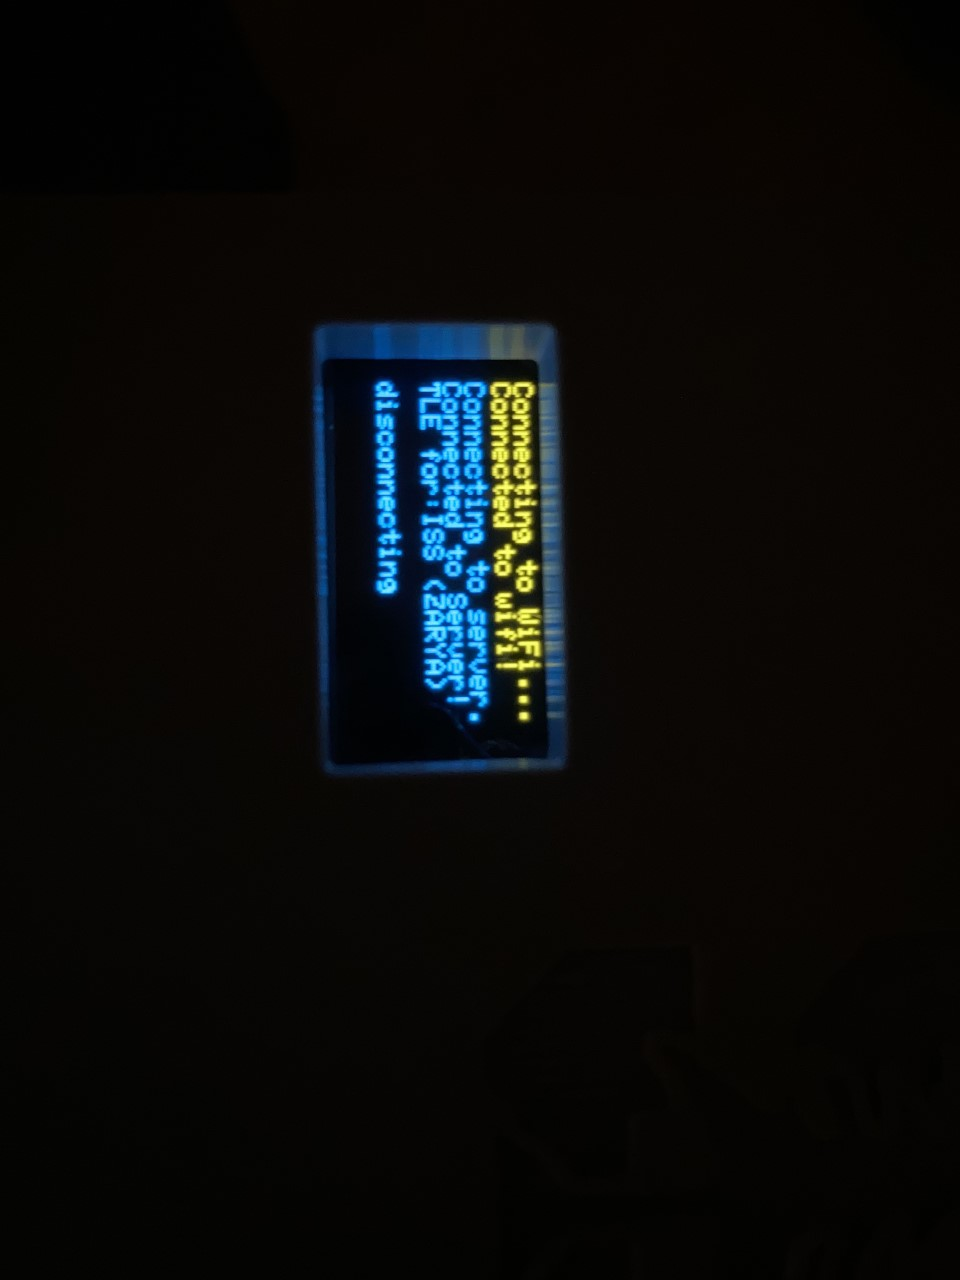
\includegraphics[width=5in]{images/OD01_Display.jpg}
			\caption{Ground Station Display}
			\label{OD01}
		\end{figure}
	    \begin{figure}[H]
		    \centering
			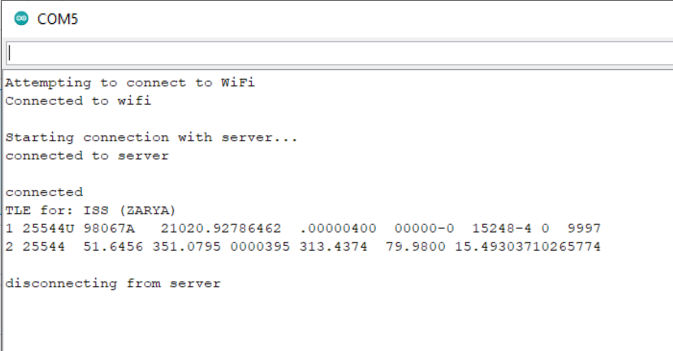
\includegraphics[width=5in]{images/SerialMonitor.png}
			\caption{Serial Monitor}
			\label{SM}
		\end{figure}
		\item \url{https://github.com/gypsyinagirl/SpacecraftDesignSchneider}
		\item (BONUS)
	\end{enumerate}
\end{enumerate}
\newpage

\section*{Problem 4}
\begin{enumerate}[label=(\alph*)]
	\item See Figure ~\ref{G}
	\begin{figure}[H]
		\centering
		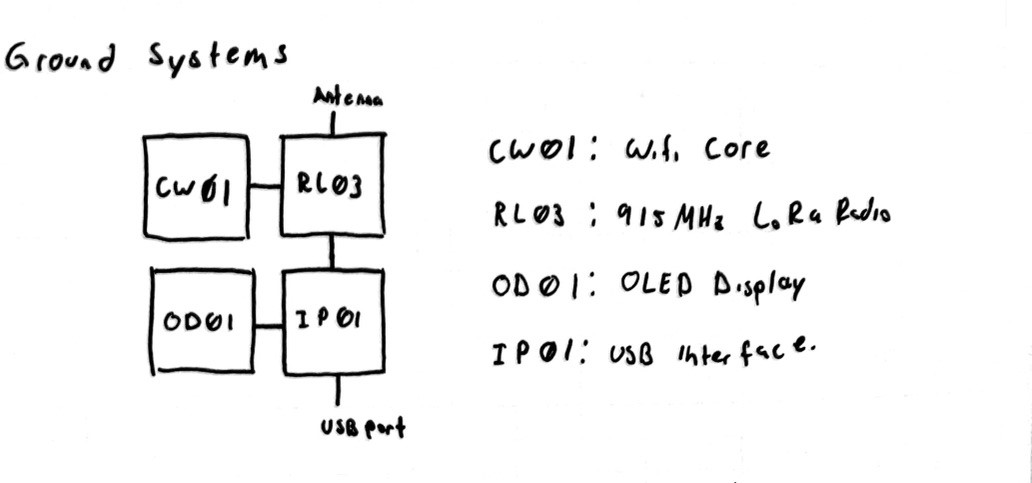
\includegraphics[width=5in]{images/Ground_station.jpg}
		\caption{Ground Station}
		\label{G}
	\end{figure}
	\item See Figure ~\ref{F}\\
	I2C:  multi-master, multi slave packet switched communication bus\\
	SPI:  single master slave communcation bus\\
	UART: sends data by bits one-by-one
	\begin{figure}[H]
		\centering
		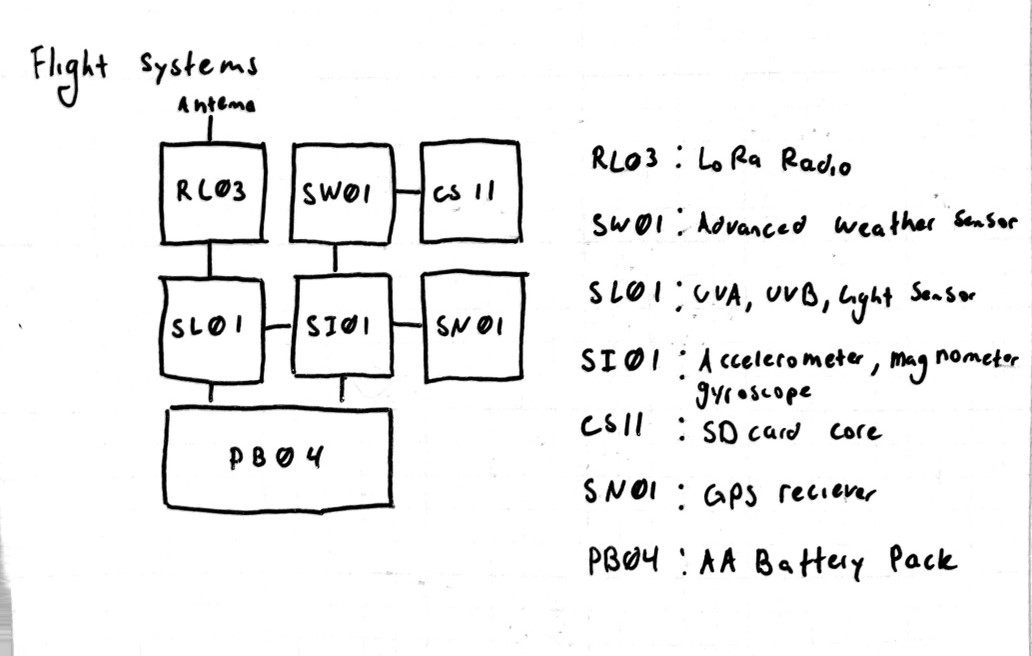
\includegraphics[width=5in]{images/Flight_station.jpg}
		\caption{Flight Station}
		\label{F}
	\end{figure}
\end{enumerate}
\end{document}
